% Modeled after sample-sigplan.tex
\documentclass[sigplan,anonymous,review,10pt]{acmart}
%% \BibTeX command to typeset BibTeX logo in the docs
\AtBeginDocument{%
  \providecommand\BibTeX{{%
    Bib\TeX}}}
\setcopyright{acmlicensed}
\copyrightyear{2018}
\acmYear{2018}
\acmDOI{XXXXXXX.XXXXXXX}
%% These commands are for a PROCEEDINGS abstract or paper.
\acmConference[Onward!]{Onward!}{Oct. 20-25, 2024}{Pasadena, CA}
\acmISBN{978-1-4503-XXXX-X/18/06}
% ============================================================
% ============================================================
\usepackage{xspace}
\usepackage{graphicx}
\graphicspath{{figures/}}
% ============================================================
%% Uncomment the next few lines to get sf url links:
%\usepackage{url}            
%\makeatletter
%\def\url@leostyle{%
%  \@ifundefined{selectfont}{\def\UrlFont{\sf}}{\def\UrlFont{\small\sffamily}}}
%\makeatother
%\urlstyle{leo} % Now actually use the newly defined style.
%% Choose coloured or b/w links:
%\usepackage[pdftex,colorlinks=true,pdfstartview=FitV,
% linkcolor=black,citecolor=black,urlcolor=black]{hyperref}
%\usepackage{hyperref}
\usepackage{needspace}
\newcommand{\needlines}[1]{\Needspace{#1\baselineskip}}
\usepackage{paralist}
% ============================================================
%:Markup macros for proof-reading
\usepackage{ifthen}
\usepackage[normalem]{ulem} % for \sout
\usepackage{xcolor}
\newcommand{\ra}{$\rightarrow$}
\newboolean{showedits}
\setboolean{showedits}{true} % toggle to show or hide edits
%\setboolean{showedits}{false} % toggle to show or hide edits
\ifthenelse{\boolean{showedits}}
{
	\newcommand{\meh}[1]{\textcolor{red}{\uwave{#1}}} % please rephrase
	\newcommand{\ins}[1]{\textcolor{blue}{\uline{#1}}} % please insert
	\newcommand{\del}[1]{\textcolor{red}{\sout{#1}}} % please delete
	\newcommand{\chg}[2]{\textcolor{red}{\sout{#1}}{\ra}\textcolor{blue}{\uline{#2}}} % please change
	\newcommand{\nbe}[3]{
		{\colorbox{#3}{\bfseries\sffamily\scriptsize\textcolor{white}{#1}}}
		{\textcolor{#3}{\sf\small$\blacktriangleright$\textit{#2}$\blacktriangleleft$}}}
}{
	\newcommand{\meh}[1]{#1} % please rephrase
	\newcommand{\ins}[1]{#1} % please insert
	\newcommand{\del}[1]{} % please delete
	\newcommand{\chg}[2]{#2}
	\newcommand{\nbe}[3]{}
}
%
\newcommand\rA[1]{\nbe{Reviewer A}{#1}{cyan}}
\newcommand\rB[1]{\nbe{Reviewer B}{#1}{olive}}
\newcommand\rC[1]{\nbe{Reviewer C}{#1}{magenta}}
\newcommand\ANS[1]{\nbe{Response}{#1}{teal}}

\newcommand{\THE}{\ins{the}\xspace} % "the" missing
\newcommand{\A}{\ins{a}\xspace} % "a" missing
\newcommand{\s}{\ins{s}\xspace} % "s" missing
\newcommand{\COMMA}{\ins{,}\xspace} % "," missing
\newcommand{\THAT}{\chg{which}{that}\xspace} % use "that", not "which"

% ============================================================
%:Box comments/edits
\usepackage[most]{tcolorbox}
\ifthenelse{\boolean{showedits}}
{
  \newtcolorbox{inserted}{%
       title=Inserted text:,
       colframe=blue,colback=blue!5!white,
       breakable,
       leftrule=0mm, 
       bottomrule=0mm,
       rightrule=0mm,
       toprule=0mm,
       arc=0mm, outer arc=0mm,
       oversize
  }
  \newtcolorbox{deleted}{%
       title=Deleted text:,
       colframe=red,colback=red!5!white,
       breakable,
       leftrule=0mm, 
       bottomrule=0mm,
       rightrule=0mm,
       toprule=0mm,
       arc=0mm, outer arc=0mm,
       oversize
  }
  \newtcolorbox{refactored}{%
       % title=Heavily modifed/refactored text:,
       title=Rewritten text:,
       colframe=blue,colback=red!5!white,
       breakable,
       leftrule=0mm, 
       bottomrule=0mm,
       rightrule=0mm,
       toprule=0mm,
       arc=0mm, outer arc=0mm,
       oversize
  }
}{
  \newenvironment{inserted}{}{}
  %\newenvironment{deleted}{ \begin{comment} }{ \end{comment} }
  \let\deleted\comment
  \newenvironment{refactored}{}{} 
}
% ============================================================
%:Put edit comments in a really ugly standout display
%\usepackage{ifthen}
%\usepackage{amssymb} % Avoid error: Command `\Bbbk' already defined.
\newboolean{showcomments}
\setboolean{showcomments}{true}
%\setboolean{showcomments}{false}
\newcommand{\id}[1]{$-$Id: scgPaper.tex 32478 2010-04-29 09:11:32Z oscar $-$}
\newcommand{\yellowbox}[1]{\fcolorbox{gray}{yellow}{\bfseries\sffamily\scriptsize#1}}
\newcommand{\triangles}[1]{{\sf\small$\blacktriangleright$\textit{#1}$\blacktriangleleft$}}
\ifthenelse{\boolean{showcomments}}
%{\newcommand{\nb}[2]{{\yellowbox{#1}\triangles{#2}}}
{\newcommand{\nbc}[3]{
 {\colorbox{#3}{\bfseries\sffamily\scriptsize\textcolor{white}{#1}}}
 {\textcolor{#3}{\sf\small$\blacktriangleright$\textit{#2}$\blacktriangleleft$}}}
 \newcommand{\version}{\emph{\scriptsize\id}}}
{\newcommand{\nbc}[3]{}
 \newcommand{\version}{}}
\newcommand{\nb}[2]{\nbc{#1}{#2}{orange}}
\newcommand{\here}{\yellowbox{$\Rightarrow$ CONTINUE HERE $\Leftarrow$}}
\newcommand\rev[2]{\nb{TODO (rev #1)}{#2}} % reviewer comments
\newcommand\fix[1]{\nb{FIX}{#1}}
\newcommand\todo[1]{\nb{TO DO}{#1}}
%\newcommand\XXX[1]{\nbc{XXX}{#1}{brown}}
%\newcommand\XXX[1]{\nbc{XXX}{#1}{cyan}}
%\newcommand\XXX[1]{\nbc{XXX}{#1}{darkgray}}
%\newcommand\XXX[1]{\nbc{XXX}{#1}{gray}}
%\newcommand\XXX[1]{\nbc{XXX}{#1}{magenta}}
%\newcommand\XXX[1]{\nbc{XXX}{#1}{olive}}
%\newcommand\XXX[1]{\nbc{XXX}{#1}{orange}}
%\newcommand\XXX[1]{\nbc{XXX}{#1}{purple}}
%\newcommand\XXX[1]{\nbc{XXX}{#1}{red}}
%\newcommand\XXX[1]{\nbc{XXX}{#1}{teal}}
%\newcommand\XXX[1]{\nbc{XXX}{#1}{violet}}
% ============================================================
\newboolean{isblinded}
\setboolean{isblinded}{true}
%\setboolean{isblinded}{false}
\ifthenelse{\boolean{isblinded}}
{\newcommand\blind[1]{BLINDED\xspace}}
{\newcommand\blind[1]{#1\xspace}}
% ============================================================
\newcommand{\seclabel}[1]{\label{sec:#1}}
%\newcommand{\secref}[1]{Section~\ref{sec:#1}} <- use \autoref instead!
\newcommand{\figlabel}[1]{\label{fig:#1}}
%\newcommand{\figref}[1]{Figure~\ref{fig:#1}}
\newcommand{\tablabel}[1]{\label{tab:#1}}
%\newcommand{\tabref}[1]{Table~\ref{tab:#1}}
% ============================================================
\newcommand{\ie}{\emph{i.e.},\xspace}
\newcommand{\eg}{\emph{e.g.},\xspace}
\newcommand{\etal}{\emph{et al.}\xspace}
\newcommand{\etc}{\emph{etc.}\xspace}
% ============================================================

% $Author: oscar $
% $Date: 2009-11-06 14:37:12 +0100 (Fri, 06 Nov 2009) $
% $Revision: 29604 $
%=============================================================
% ST80 listings macros
% Adapted from Squeak by Example book
%=============================================================
% If you want >>> appearing as right guillemet, you need these two lines:
%\usepackage[T1]{fontenc}
%\newcommand{\sep}{\mbox{>>}}
% Otherwise use this:
\newcommand{\sep}{\mbox{$\gg$}}
%=============================================================
%:\needlines{N} before code block to force page feed
%\usepackage{needspace}
%\newcommand{\needlines}[1]{\Needspace{#1\baselineskip}}
%=============================================================
%:Listings package configuration for ST80
\usepackage[english]{babel}
%\usepackage{amssymb,textcomp}
\usepackage{listings}
% \usepackage[usenames,dvipsnames]{color}
% \usepackage[usenames]{color}
% \definecolor{source}{gray}{0.95}
\lstdefinelanguage{Smalltalk}{
  % morekeywords={self,super,true,false,nil,thisContext, eachModel}, % This is overkill
  morestring=[d]',
  morecomment=[s]{"}{"},
  alsoletter={\#:},
  escapechar={!},
  literate=
    {BANG}{!}1
    {UNDERSCORE}{\_}1
    % {\\st}{Smalltalk}9 % convenience -- in case \st occurs in code
    % {'}{{\textquotesingle}}1 % replaced by upquote=true in \lstset
    {_}{{$\leftarrow$}}1
    {>>>}{{\sep}}1
    {^}{{$\uparrow$}}1
    {~}{{$\sim$}}1
    {-}{{\sf -\hspace{-0.13em}-}}1  % the goal is to make - the same width as +
    {+}{\raisebox{0.08ex}{+}}1		% and to raise + off the baseline to match -
    {-->}{{\quad$\longrightarrow$\quad}}3
	, % Don't forget the comma at the end!
  tabsize=4
}[keywords,comments,strings]

\definecolor{source}{gray}{0.95}

\lstset{language=Smalltalk,
	basicstyle=\sffamily,
	keywordstyle=\color{black}\bfseries,
%	numbers=left,                   % where to put the line-numbers
%	numberstyle=\footnotesize,      % the size of the fonts that are used for the line-numbers
%	stepnumber=1,                   % the step between two line-numbers. If it is 1 each line will be numbered
%	numbersep=5pt,                  % how far the line-numbers are from the code
%	stringstyle=\ttfamily, % Ugly! do we really want this? -- on
	mathescape=true,
	showstringspaces=false,
	keepspaces=true,
	breaklines=true,
	breakautoindent=true,
	backgroundcolor=\color{source},
	%lineskip={-1pt}, % Ugly hack
	upquote=true, % straight quote; requires textcomp package
	columns=fullflexible} % no fixed width fonts
% In-line code (literal)
% Normally use this for all in-line code:
\newcommand{\st}{\lstinline[mathescape=false,backgroundcolor=\color{white},basicstyle={\sffamily\upshape}]}
% In-line code (latex enabled)
% Use this only in special situations where \ct does not work
% (within section headings ...):
\newcommand{\lst}[1]{{\textsf{\textup{#1}}}}
% Code environments
\lstnewenvironment{code}{%
	\lstset{%
		% frame=lines,
		frame=single,
		framerule=0pt,
		mathescape=false
	}
}{}

% Useful to add a matching $ after code containing a $
% \def\ignoredollar#1{}
%=============================================================

% ============================================================
% Macros for this paper
%\renewcommand{\nbc}[3]{} % To hide reviewer comments
\newcommand\on[1]{\nbc{ON}{#1}{olive}} % add more author macros here
\newcommand\tg[1]{\nbc{TG}{#1}{blue}}
%\newcommand\XXX[1]{\nbc{XXX}{#1}{red}}
%\newcommand\XXX[1]{\nbc{XXX}{#1}{teal}}
%\newcommand\XXX[1]{\nbc{XXX}{#1}{violet}}
\usepackage{caption}
\captionsetup{aboveskip=5pt,belowskip=-10pt} % Adjust the space around figure captions
%\usepackage{enumitem}
%\setlist[description]{font=\itshape}
\newcommand{\GT}{\lst{GT}\xspace} % In case we want to display it differently ...
% ============================================================
% Optionally anonymize selected names
\newboolean{anonymous}
\setboolean{anonymous}{true}
\newcommand\anonymize[2]{\ifthenelse{\boolean{anonymous}}{#2}{#1}\xspace}
\newcommand\feenk{\anonymize{feenk}{anonymous company}}
% ============================================================
\begin{document}
\title{Moldable Exceptions}
\author{Andrei Chi\c{s}}
\affiliation{%
  \institution{feenk gmbh}
  \city{Wabern}
  \country{Switzerland}}
\email{andrei.chis@feenk.com}
%\author{Tudor G\^irba}
%\affiliation{%
%  \institution{feenk gmbh}
%  \city{Wabern}
%  \country{Switzerland}}
%\email{tudor.girba@feenk.com}
\author{Oscar Nierstrasz}
\affiliation{%
  \institution{feenk gmbh}
  \city{Wabern}
  \country{Switzerland}}
\email{oscar.nierstrasz@feenk.com}

\renewcommand{\shortauthors}{Chi\c{s} et al.}

\begin{abstract}
\todo{DRAFT}
Debugging is hard.
All debuggers are the same.
They show you a stack, a way to sample the state of the stack, and, if the debugger is live, a way to step through execution.
Exceptions are always raised in a specific context.
We can exploit this context to show more useful information when debugging.
Moldable exceptions offer a lightweight mechanism to adapt a moldable debugger to the specific context of the exception raised to show more useful views and actions to a developer.
We present, through a series of examples, how moldable exceptions can be added to a live programming environment.
\end{abstract}


\keywords{\todo{}}

%\received{20 February 2007}
%\received[revised]{12 March 2009}
%\received[accepted]{5 June 2009}

\maketitle

% ============================================================
\section{Introduction}\label{sec:intro}

\todo{Just a rough outline --- text to be rewritten}

In the bad old days, all debuggers were the same.
You had commands to sample the current execution state, and you had commands to step through the running code.
Nowadays we have graphical debuggers that show us the run-time stack, and offer buttons instead of commands to step through the code, but they are still all the same.
The trouble with this is that every debugging problem is different, but debuggers all show us the same thing.

What if the debugger were to be aware of the kind of exception being raised, and instead of showing a generic debugger view, it would provide views and actions specific to the context of that exception?
This is what \emph{moldable exceptions} do.

\todo{Explain the example}

\begin{figure}[h]
  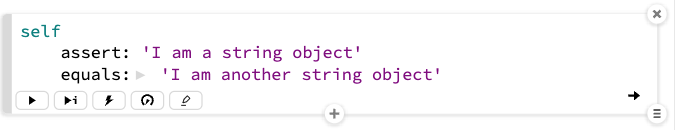
\includegraphics[width=\columnwidth]{stringComparisonSnippet}
  \caption{A failing string comparison assertion.}
  \label{fig:stringComparisonSnippet}
\end{figure}

\begin{figure}[h]
  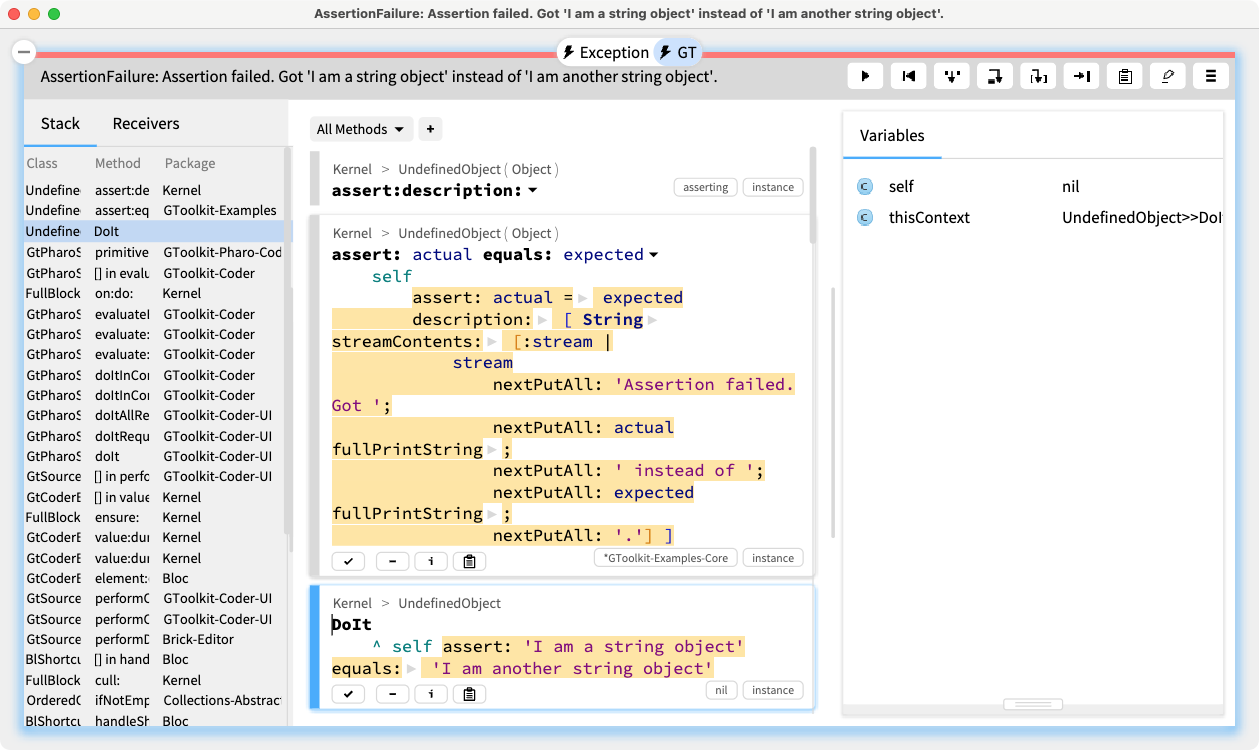
\includegraphics[width=\columnwidth]{genericDebugger}
  \caption{A generic debugger view.}
  \label{fig:genericDebugger}
\end{figure}

\begin{figure}[h]
  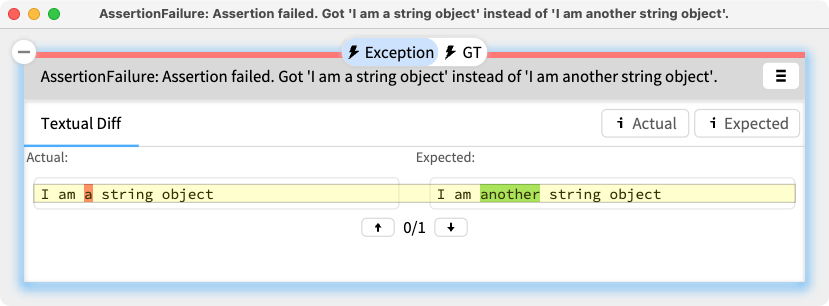
\includegraphics[width=\columnwidth]{stringComparisonView}
  \caption{A string diff debugger view.}
  \label{fig:stringComparisonView}
\end{figure}

Moldable exceptions work as follows: when an exception is raised, the exception (an object) is caught and passed to the debugger.
Every exception not only provides the debugger with the context it needs to generate the debugging UI, but it can also offer alternative views and actions.
In the case of our implementation, this is achieved by the exception class providing specially annotated debugger extension methods.

This simple mechanism allows moldable exceptions to do three things:
\begin{inparaenum}[(i)]
	\item provide domain-specific debugging views and actions,
	\item offer new debugger GUI interactions, and
	\item enable automated fixes (code transformations) for common programming errors.
\end{inparaenum}    

\todo{add section overview}
In \autoref{sec:views} we will ...
\autoref{sec:interactions}
\autoref{sec:fixes}
\autoref{sec:directions}
We discuss related work in \autoref{sec:related}.
We conclude in \autoref{sec:conclusion}.

% ============================================================
\section{Adding views and actions}\label{sec:views}

\todo{
This should function like a mini-tutorial, where we add debugger views to an existing class.
We could use the Ludo game as a first example.
Then we proceed to the assertion diff example, which looks at the context.
}

% ============================================================
\section{Providing domain-specific debugger interactions}\label{sec:interactions}

\todo{
Collector views.
Mention other domains from the moldable debugger, such as event-driven apps and parsers?
}

% ============================================================
\section{Enabling automated fixes}\label{sec:fixes}

\todo{
Introduce the deprecation special case.
Demo the empty view fix example.
Discuss the LifeWare tests?
}

% ============================================================
\section{Future directions}\label{sec:directions}

\todo{
Providing views with access to the debugger context.
Moldable exceptions for other platforms -- what do you need?
}

% ============================================================
\section{Related work}\label{sec:related}

\todo{Expand this list}

Moldable Debugger
\cite{Chis15c}

On the Dichotomy of Debugging Behavior Among Programmers
\cite{Bell18a}
Online developer survey shows that IDE-provided debuggers are not used as often as expected.

A Simple and Extensible Graphical Debugger
\cite{Hans97a}
An early example of an extensible debugger

Grammar-Driven Generation of Domain-Specific Language Debuggers
\cite{HuiW08a}
Generating debuggers for DSLs from the grammar spec.

Declaratively Defining Domain-Specific Language Debuggers
\cite{Lind11a}
Using a high-level spec to define DSL debuggers


% ============================================================
\section{Conclusion}\label{sec:conclusion}

\todo{xxx}


%% The acknowledgments section is defined using the "acks" environment
%% (and NOT an unnumbered section).
%\begin{acks}
%To Robert, for the bagels and explaining CMYK and color spaces.
%\end{acks}

\bibliographystyle{ACM-Reference-Format}
\bibliography{moldableExceptions}


\end{document}
\endinput

